\documentclass[11pt,oneside]{article}
\special{papersize=8.5in,11in}
\usepackage  {graphics}
%\usepackage {harvard}
\usepackage[round]{natbib}
\usepackage{graphicx,color}
\usepackage{verbatim}
\usepackage{subfigure}
\usepackage{epsfig}
\usepackage{latexsym}
\usepackage{longtable}
\usepackage{rotating}
\usepackage{multirow}
\usepackage{wrapfig}
%\usepackage{slashbox}
\usepackage{float}
\usepackage{amsmath}
\usepackage{amssymb}
\usepackage{amsthm}
%\usepackage{times}
\usepackage{multirow}
\usepackage{footnote}
\usepackage{lineno}
\usepackage{authblk}
\usepackage[sc]{mathpazo}
\usepackage{lineno}
\usepackage{xcolor}
\usepackage{tikz}
\usetikzlibrary{positioning,arrows.meta,fit,backgrounds,calc}
\linespread{1.05}
%\usepackage[nomarkers]{endfloat}
 %\usepackage[sc]{mathpazo}
 %\linespread{1.05}
%\setlength{\parindent}{2.5em}
%\setlength{\parskip}{1em}
%%%%%%%%%% EXACT 1in MARGINS %%%%%%%                                   %%
\setlength{\textwidth}{6.5in}     %%                                   %%
\setlength{\oddsidemargin}{0in}   %% (It is recommended that you       %%
\setlength{\evensidemargin}{0in}  %%  not change these parameters,     %%
\setlength{\textheight}{9in}      %%  at the risk of having your       %%0
%\setlength{\topmargin}{0.5in}       %%  proposal dismissed on the basis  %%
\setlength{\headheight}{-0.4in}      %%  of incorrect formatting!!!)      %%
\setlength{\headsep}{0.1in}         %%                                   %%

\newtheorem{proposition}{Proposition}
\newtheorem{theorem}{Theorem}
\newtheorem{lemma}{Lemma}
\newtheorem{definition}{Definition}
\newtheorem{corollary}{Corollary}
\newtheorem{assumption}{Assumption}
\newcommand{\refeqn}[1]{(\ref{#1})}
\newcommand{\refeqnf}[1]{Eqn. (\ref{#1})}
\newcommand{\reffig}[1]{Figure \ref{#1}}
\newcommand{\reftab}[1]{Table \ref{#1}}

\newenvironment{WhileBlock}[1]{
%    \vspace{-2pt}
  \begin{flushleft}  {\vspace*{-12pt}While (#1)} \end{flushleft}
  \vspace{-10pt}
    \begin{itemize}
 }
 {
    \end{itemize}
 \begin{flushleft}  {\vspace*{-15pt}End while} \end{flushleft}
    %\vspace{6pt}
}

\newenvironment{ForBlock}[1]{
%    \vspace{-2pt}
  \begin{flushleft}  {\vspace*{-6pt}For #1} \end{flushleft}
  %\vspace{-10pt}
    \begin{itemize}
 }
 {
    \end{itemize}
  \begin{flushleft}  {\vspace*{-15pt}End for} \end{flushleft}
    %\vspace{6pt}
}

\newenvironment{IfBlock}[1]{
%    \vspace{-2pt}
  \begin{flushleft}  {\vspace*{-6pt}If (#1)} \end{flushleft}
  %\vspace{-10pt}
    \begin{itemize}
 }
 {
    \end{itemize}
  \begin{flushleft}  {\vspace*{-6pt}End if} \end{flushleft}
    %\vspace{6pt}
}
\newenvironment{IfBlockOpen}[1]{
%    \vspace{-2pt}
  \begin{flushleft}  {\vspace*{-6pt}If (#1)} \end{flushleft}
  \vspace{-10pt}
    \begin{itemize}
 }
 {
    \end{itemize}
    %\vspace{6pt}
}
\newenvironment{ElseBlock}{
%    \vspace{-2pt}
  \begin{flushleft}  {\vspace*{-12pt}Else} \end{flushleft}
  \vspace{-10pt}
    \begin{itemize}
 }
 {
    \end{itemize}
  \begin{flushleft}  {\vspace*{-12pt}End if} \end{flushleft}
    %\vspace{6pt}
}
\newcommand{\ProgramBlock}[1]{
    \vspace{-6pt}
     \item []  #1
}

\newenvironment{AlgorithmSteps}[1]{
%    \vspace{-2pt}
  \begin{flushleft}  {\vspace*{-6pt}\fontfamily{phv}\selectfont\scshape Algorithm #1} \end{flushleft}
  \vspace{-10pt}
    \begin{itemize}
 }
 {
    \end{itemize}
    %\vspace{6pt}
}
\newcommand{\AlgorithmStepItem}[2]{
    \vspace{-5pt}
     \item []\hspace{-30pt} \textbf{Step #1}\hspace{5pt}  #2
}
\newcommand{\AlgorithmSubStepItem}[2]{
    \vspace{-8pt}
     \item []\hspace{0pt}\textit{Step #1}\hspace{5pt}  #2
}
\newcommand{\TRBSubmitPresent}[3]{\vspace*{20pt}\begin{center}Submitted to \textit{#2} Committee (\textbf{#3})\\for Presentation at the #1 Annual Meeting of Transportation Research
Board\end{center}}
\newcommand{\TRBSubmitPublish}[3]{\vspace*{20pt}\begin{center}Submitted to \textit{#2} Committee (\textbf{#3})\\for Presentation at the #1 Annual Meeting of Transportation Research
Board and \\for Publication in the Journal of Transportation
Research Record\end{center}}
\newcommand{\citeeg}[1]{
   (e.g. \cite{#1})}
   \newcommand{\citeaf}[2]{
   (#2 \cite{#1})}
   \newcommand{\TRBwordcounts[5]}{\vspace*{20pt}\begin{center}Word counts based on Translator's Abacus on the PDF File\\ \texttt{#2} words + \texttt{#3} tables + \texttt{#4} figures = \texttt{#5}\end{center}}



\begin{document}
\pagewiselinenumbers
\baselineskip=15pt %This means double space
\title{On the Allocation of Humannoid Robots in a Ride-Parcel-Pooling Service with Robot Taxis }
%OLD: \author{Yang Liu, Yu (Marco) Nie\footnote{Corresponding author} and Jonathan Hall\\Department of Civil and Environmental Engineering\\Northwestern University, 2145 Sheridan Road, Evanston, IL 60208\\Email: y-nie@northwestern.edu\\Phone: 1-847-467-0502}

%ADDED: Goal was just to have my affiliation listed, this was the best way I could figure out how to do so without adding a package
% \author[1]{Yang Zhenyu}
% \author[2]{Yu (Marco) Nie \footnote{Corresponding author, Phone: 1-847-467-0502; Email: y-nie@northwestern.edu}}
% \author[3]{Jonathan Hall}
% \affil[1]{Department of Industrial and Systems Engineering, National University of Singapore, Singapore}
% \affil[2]{Department of Civil and Environmental Engineering, Northwestern University, Evanston, Illinois}
% \affil[3]{Department of Economics and School of Public Policy and Governance, University of Toronto,  Toronto}




\maketitle\begin{abstract}

Humanoid robots are gradually being deployed in various service industries, including urban transportation. While vehicle automation removes the need for human drivers, many non-driving tasks traditionally performed by drivers still need to be addressed, creating a potential role for humanoid robots. This paper envisions a future scenario where humanoid robots are integrated into ride-parcel-pooling services, providing both passenger transportation and parcel delivery. We investigate the allocation of humanoid robots in a ride-parcel-pooling service, where the same robot fleet can perform passenger- and parcel-related tasks over time. We develop a mathematical model to optimize robot allocation while minimizing operational costs. The model considers factors such as demand patterns, robot availability, and task constraints. We also propose an algorithm to solve the allocation problem and demonstrate its effectiveness through numerical experiments. The results provide insights into the optimal deployment strategies for humanoid robots in shared mobility services, highlighting the potential benefits of integrating robotic assistance in urban transportation systems.
\\
\textit{Keywords}: Ridesharing, Humanoid Robots, Resource Allocation
\end{abstract}


\section{Introduction}

Autonomous driving is expected to remove the need for human drivers in ride-hailing and shared mobility systems. However, eliminating drivers does not eliminate the many non-driving tasks that drivers currently perform, such as boarding assistance for passengers with reduced mobility, parcel handover and verification, curbside coordination, and basic exception handling at pickup and drop-off points. As autonomous fleets scale up, this operational gap becomes increasingly urgent and can directly limit service quality and system throughput. In this context, humanoid robots become a practical substitute for driver-side labor, enabling autonomous mobility systems to support passenger- and parcel-related tasks without relying on onboard human staff.

As shown in Fig. \ref{fig:robot_rpp}, the proposed task-allocation system integrates multiple mobility and logistics functions within a shared urban network. The diagram illustrates three representative task categories: passenger assistance, parcel delivery, and station operation. Vehicles, robots, public transport stations, and users are connected through coordinated routes, where solid arrows indicate vehicle or robot movements and dotted arrows represent station-related task flows. Passenger-assistance tasks support users with mobility needs at pick-up and drop-off nodes. Parcel-chain tasks enable robots and vehicles to cooperate in transferring packages across different locations. Station-operation tasks provide time-block robot support for public transport stations, such as passenger guidance, crowd management, and congestion mitigation. Together, these interconnected components demonstrate how the system can support both human-centered mobility and goods transportation in a unified operational framework.

\begin{figure}[ht!]
  \centering
  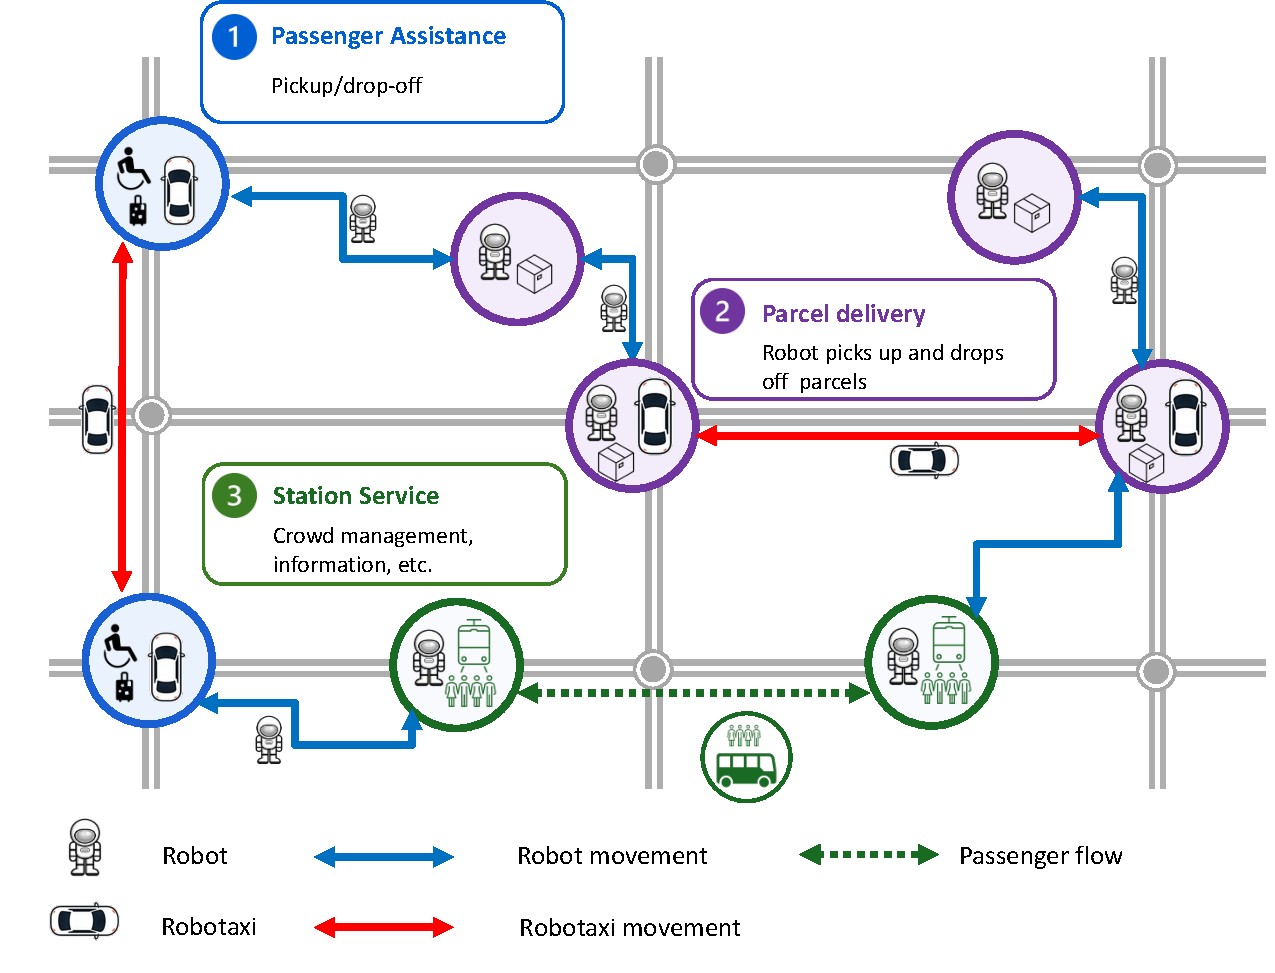
\includegraphics[width=1\textwidth,keepaspectratio]{figs/framework.pdf}
  \caption{Illustration of the robot assisted RPP system}
  \label{fig:robot_rpp}
\end{figure}

% We consider the humanoid robots are provided by a robot taxi company, which is responsible for the operation and maintenance of the robots. The robot taxi company can deploy humanoid robots to serve passengers and parcels in a ride-parcel-pooling service. The service can be designed to accommodate both passenger transportation and parcel delivery, allowing for efficient utilization of the humanoid robots.

% Here, we consider two types of services that humanoid robots can provide in a ride-parcel-pooling service with AVs. 

% \begin{itemize}
%   \item  \textbf{Passenger Transportation}: Humanoid robots can can assist passengers with reduced mobility with boarding and alighting.
%   \item \textbf{Parcel Transportation}: Humanoid robots can can assist with parcel delivery and pickup.
% \end{itemize}

\section{Humanoid Robot Allocation Model}

\subsection{Robot Tasks and Information Structure}

We consider a robot company that operates a set \(K\) of
humanoid robots and provides Robot-as-a-Service to ride-hailing and public transport
clients. Let \(N\) denote the set of task nodes, \(V\) the set of linked
ride-hailing vehicles,
and \(I_t\) the set of robot tasks that are available at decision time
point \(t\). Robot movement between nodes \(m,n\in N\) is represented by the
travel time \(\tau_{mn}\) for any \(m,n\in N\).

Each task \(i\in I_t\)  is represented by
\[
i=
\left(
q_i,n_i,r_i,d_i,s_i,R_i
\right).
\]
Here, \(q_i\) is the task category, \(n_i\in N\) is the single node at which
the task is performed, \(r_i\) and \(d_i\) are its release and due times,
\(s_i\) is its duration, and \(R_i\) is its revenue. No within-task inter-node
movement is modeled. An operation involving multiple nodes is decomposed into
linked single-node tasks, and robot movement between consecutive tasks is
represented by \(\tau_{mn}\).

We consider three task categories, so that
\[
q_i\in\{\mathrm{A},\mathrm{C},\mathrm{S}\},
\]
where \(\mathrm{A}\), \(\mathrm{C}\), and \(\mathrm{S}\) denote
passenger-assistance, parcel-chain, and station-operation tasks, respectively.

Category-specific information is defined separately instead of being grouped
in a general requirement vector. Let \(I_t^{\mathrm V}\subseteq I_t\) denote
the set of tasks requiring synchronization with a ride-hailing vehicle. For
each \(i\in I_t^{\mathrm V}\), \(v_i\in V\) is the linked vehicle and \(e_i\)
is its expected arrival time at \(n_i\). Let
\(I_t^{\mathrm C}=\{i\in I_t:q_i=\mathrm C\}\). For each parcel-chain task
\(i\in I_t^{\mathrm C}\), \(p_i\) is the parcel identifier and
\(\mathcal P_i\) is the set of predecessor tasks that must be completed before
task \(i\) can start. Station-operation tasks require no additional attribute:
their fixed contractual interval is specified directly by \(r_i\) and \(d_i\).
The three categories are described below.

\noindent\textbf{Passenger-assistance task
\((q_i=\mathrm{A})\).}
A passenger-assistance task supports passenger boarding or alighting at a
ride-hailing pick-up or drop-off node. It is generated in real time after the
ride-hailing request is confirmed and the assigned vehicle, task node, and
expected vehicle arrival time become observable. The task is performed at
node \(n_i\), and its linked vehicle \(v_i\) and expected arrival time \(e_i\)
define the synchronization requirement. The assigned robot travels to the node
and must be ready in coordination with the vehicle.

\noindent\textbf{Parcel-chain task
\((q_i=\mathrm{C})\).}
The  origins and destinations of parcel delivery requests are known
at the beginning of the day, but their executable robot tasks are
activated only after the RPP system specifies the relevant task nodes and
expected handover times. Each pickup, handover, or delivery operation is
represented as a separate single-node task. Tasks belonging to the same parcel
share the identifier \(p_i\) and are ordered by their predecessor sets
\(\mathcal P_i\). A parcel task that involves vehicle handover also belongs to
\(I_t^{\mathrm V}\) and therefore has linked-vehicle data \((v_i,e_i)\). The
tasks may be assigned to different robots but retain the common category
\(q_i=\mathrm{C}\). Robot movement between their nodes is represented by
\(\tau_{mn}\). The set \(P_t\) contains known parcel requests that have not
yet been activated by an RPP matching result.



\noindent\textbf{Station-operation task
\((q_i=\mathrm{S})\).}
A station-operation task is a long-duration task block at a fixed public
transport station for passenger guidance, flow management, or congestion
mitigation. Its station node, contractual start and end times, and required
number of robots are known at the beginning of the day. Each required robot is
represented by one atomic task, and once the task is assigned, its
task interval is locked in the robot schedule as a hard commitment.

\begin{table}[htbp]
\centering
\caption{Illustrative task data for three categories (Munich city-center example).}
\label{tab:task_tuple_examples}
\resizebox{\textwidth}{!}{%
\begin{tabular}{l l l l l l l}
\hline
$q_i$ & $n_i$ & $r_i$ & $d_i$ & $s_i$ & $R_i$ & Category-specific data \\
\hline
$\mathrm{A}$ & Marienplatz & 08:12 & 08:20 & 5 min & 14 & $v_i=v_{231}$; $e_i=08{:}15$ \\
$\mathrm{C}$ & Munich Hbf & 09:05 & 09:35 & 12 min & 18 & $p_i=p_{77}$; $\mathcal P_i=\{j\}$; $v_i=v_{118}$; $e_i=09{:}20$ \\
$\mathrm{S}$ & Karlsplatz (Stachus) & 07:00 & 10:00 & 180 min & 95 & fixed contract interval $[r_i,d_i]$ \\
\hline
\end{tabular}%
}
\end{table}

\subsection{Markov Decision Process Formulation}

The allocation problem is formulated over a finite operating day with
decision time points \(t\in\mathcal T\). A decision time point is triggered by
the beginning of the day, the arrival of a new passenger-assistance task,
an RPP matching result, the completion of a robot task, or a material
update of a linked vehicle's expected arrival time.

\subsubsection{State}

The system state is
\[
S_t=
\left(
t,\boldsymbol{\ell}_t,\boldsymbol{b}_t,
\boldsymbol{\pi}_t,I_t,P_t,E_t,B
\right).
\]
Here, \(\ell_{kt}\) and \(b_{kt}\) denote the current node and earliest
available time of robot \(k\), respectively;
\(\boldsymbol{\pi}_t=(\pi_{kt})_{k\in K}\) is the collection of current robot
schedules; \(I_t\) is the active task set; \(P_t\) is the set of known but
not-yet-activated parcel requests; \(E_t\) contains the currently observed RPP
vehicle assignments and arrival-time information; and \(B\) is the set of
station-operation commitments known at the beginning of the day. Although
\(I_t\) is a component of \(S_t\), it is written separately below when useful
to emphasize the tasks considered by the online assignment decision.

\subsubsection{Action and Feasibility}

Let \(x_{ik}^t\in\{0,1\}\) indicate whether task \(i\) is assigned to
robot \(k\) at time point \(t\), and let \(\pi'_{kt}\) denote the updated
ordered schedule of robot \(k\). An action is
\[
\nu_t=
\left(
x_t,\boldsymbol{\pi}'_t
\right).
\]
The feasible action set is compactly written as
\[
\mathcal U(S_t)=
\left\{
\begin{array}{ll}
(x_t,\boldsymbol{\pi}'_t):&
\displaystyle \sum_{k\in K}x_{ik}^t\leq 1,
\quad \forall i\in I_t,\\[2mm]
&
x_{ik}^t\in\{0,1\},
\quad \forall i\in I_t,\ k\in K,\\[1mm]
&
\pi'_{kt}\in\Pi_k(S_t),
\quad \forall k\in K,\\[1mm]
&
x_{ik}^t=1\ \Longrightarrow\ i\in\pi'_{kt}
\end{array}
\right\}.
\]
The set \(\Pi_k(S_t)\) embeds robot availability, task ordering,
node-to-node travel times, release and due times, task durations, vehicle
synchronization, parcel-chain precedence, and all previously locked
commitments. Tasks already
being executed cannot be reassigned. Station-operation tasks are represented as
atomic units and must satisfy
\[
\sum_{k\in K}x_{ik}^0=1,
\qquad \forall i\in B,
\]
at the beginning of the day; once assigned, their specified task intervals
remain fixed in the corresponding robot schedules.

The timing of an assigned task is induced by its robot schedule:
\[
a_i=a_i(\pi'_{kt},S_t),
\qquad
c_i=c_i(\pi'_{kt},S_t),
\qquad
L_i=\left[c_i(\pi'_{kt},S_t)-d_i\right]^+.
\]
Thus, \(a_i\), \(c_i\), and \(L_i\) are outcomes rather than input attributes.
Station-operation and parcel-chain requirements are imposed directly as
\[
a_i=r_i,\quad c_i=d_i,
\qquad \forall i\in B,
\]
\[
a_i\geq c_j,
\qquad
\forall i\in I_t^{\mathrm C},\ j\in\mathcal P_i.
\]
For a synchronized task, if \(u_i\) is the robot-ready time induced by the
schedule and \(e_i\) is the linked vehicle arrival time, then
\[
a_i=\max\{u_i,e_i\},
\qquad
W_i^r=[e_i-u_i]^+,
\qquad
W_i^v=[u_i-e_i]^+.
\]

\subsubsection{Stochastic Information and State Transition}

Let
\[
\zeta_{t+1}=
\left(
A_{t+1},M_{t+1},E_{t+1},\tau_{t+1}
\right)
\]
denote the new information observed before the next decision time point.
Here, \(A_{t+1}\) contains new passenger-assistance tasks,
\(M_{t+1}\) contains new RPP matching outcomes for pending parcels,
\(E_{t+1}\) contains vehicle-arrival updates, and \(\tau_{t+1}\) contains
updated or realized travel-time information. If \(\Gamma(M_{t+1})\) denotes
the parcel tasks activated by the new matching outcomes and \(D_t\)
denotes completed or expired tasks, the active set evolves according to
\[
I_{t+1}
=
\left(I_t\setminus D_t\right)
\cup A_{t+1}
\cup\Gamma(M_{t+1}).
\]
The full state transition is written as
\[
S_{t+1}=F(S_t,\nu_t,\zeta_{t+1}),
\]
where \(F(\cdot)\) also updates robot locations, availability, schedules,
pending parcels, and vehicle information. The state is assumed to contain all
information required for the transition distribution, so that
\[
\Pr(S_{t+1}\mid S_0,\nu_0,\ldots,S_t,\nu_t)
=
\Pr(S_{t+1}\mid S_t,\nu_t).
\]

\subsubsection{One-Step Cost}

Let
\(\widetilde T_t\), \(\widetilde W_t^r\), \(\widetilde W_t^v\),
\(\widetilde L_t\), \(\widetilde U_t\), and \(\widetilde R_t\) denote the
normalized robot travel cost, robot waiting cost, vehicle waiting cost,
lateness cost, unserved-task cost, and collected revenue during the
transition from \(t\) to \(t+1\), respectively. The one-step cost is
\[
C(S_t,\nu_t,\zeta_{t+1})
=
\widetilde T_t
+\widetilde W_t^r
+\widetilde W_t^v
+\widetilde L_t
+\widetilde U_t
-\widetilde R_t.
\]
The normalization incorporates the economic values assigned by the robot
operator; in particular, one minute of vehicle waiting is assigned a larger
normalized cost than one minute of robot waiting. These normalization
constants, as well as travel times, task durations, vehicle arrival times, and
contract values, are model inputs rather than heuristic parameters.

\subsubsection{Bellman Equation}

Let \(V_t(S_t)\) be the minimum expected cost from time point \(t\) to the end
of the operating day. The exact optimality equation is
\[
V_t(S_t)
=
\min_{\nu_t\in\mathcal U(S_t)}
\mathbb E
\left[
C(S_t,\nu_t,\zeta_{t+1})
+V_{t+1}\!\left(F(S_t,\nu_t,\zeta_{t+1})\right)
\mid S_t,\nu_t
\right],
\]
with terminal value
\[
V_{T+1}(S_{T+1})=\widetilde U_{T+1},
\]
where the terminal cost accounts for tasks that remain unserved at the
end of the day. A policy \(\mu\) maps each observed state to a feasible action,
\[
\nu_t=\mu(S_t),
\]
and the optimal policy is the policy induced by the Bellman equation. Because
the action depends only on information contained in \(S_t\), decisions cannot
use passenger requests or RPP matching outcomes that have not yet been
observed.

The compact assignment expression introduced above,
\[
\min_{x,\pi}
\sum_{i\in I_t}\sum_{k\in K}
x_{ik}G_i(k,\pi_k)
+\Phi(S_{t+1}),
\]
is a one-step representation of this Bellman equation. The assignment term
approximates the immediate cost, while
\[
\Phi(S_{t+1})
\approx
\mathbb E\!\left[V_{t+1}(S_{t+1})\mid S_t,\nu_t\right]
\]
approximates the continuation value of the resulting robot locations,
schedules, pending parcels, and remaining station commitments.

\section{Solution Approach}

\subsection{Commitment-Aware Rolling-Horizon Insertion Heuristic}

Solving the Bellman equation exactly would require a state space containing
all robot schedules and a scenario tree for future passenger requests, RPP
matching outcomes, and vehicle arrival times. We therefore approximate its
one-step decision using a commitment-aware rolling-horizon insertion policy,
denoted by
\[
\nu_t=\mu_\theta(S_t,I_t).
\]
The method retains the exact feasibility set \(\Pi_k(S_t)\), but replaces the
unknown continuation value with a simple forecast-based opportunity term.

\subsubsection{Beginning-of-Day Initialization}

At \(t=0\), each robot starts from its given storage node. The station
tasks in \(B\) are processed by increasing start time and decreasing
insertion regret, inserted using the feasible-insertion rule below, and then
locked because their task intervals are contract commitments. The pending
parcel set \(P_0\) is not assigned to robots before RPP matching. Instead, it
is combined with historical passenger-assistance demand to construct
\(p_{nt}^{H}\), the normalized expected share of robot-task demand at
node \(n\) over the next \(H\) units of time.

\subsubsection{Feasible Insertions}

At a decision time point \(t\), the heuristic considers released tasks
whose due times lie within the rolling horizon. For every task \(i\),
robot \(k\), and insertion position \(p\), define a candidate
\[
c=(i,k,p),
\qquad
\pi_{kt}^{c}=\pi_{kt}\oplus_p i.
\]
Its feasibility set is
\[
\mathcal C_i(S_t)
=
\left\{
(i,k,p):
\pi_{kt}\oplus_p i\in\Pi_k(S_t)
\right\}.
\]
Candidate evaluation propagates timing through the remainder of the affected
schedule. Consequently, the movement from the preceding task to
\(n_i\) and the movement from \(n_i\) to the succeeding task are included. A
candidate is removed
if it would violate vehicle synchronization, an already dispatched task,
or a locked station-operation interval.

\subsubsection{Insertion Cost and Approximate Continuation Value}

For a feasible candidate \(c=(i,k,p)\), let
\(\Delta\widetilde T_c\) denote incremental robot travel,
\(\Delta\widetilde W_c^r\) and
\(\Delta\widetilde W_c^v(\delta)\) the incremental robot and vehicle waiting,
\(\Delta\widetilde L_c\) the incremental lateness propagated through the
schedule, and \(\widetilde R_i\) the normalized task revenue. The
parameter \(\delta\geq0\) is a synchronization safety buffer: for a linked
vehicle arrival estimate \(e_i\), the heuristic evaluates the risk of vehicle
waiting relative to the earlier robot-ready target \(e_i-\delta\). In
particular, if \(u_c\) is the robot-ready time under candidate \(c\), the
risk-adjusted vehicle-waiting term is based on
\[
\widehat W_c^v(\delta)
=
\left[u_c-(e_i-\delta)\right]^+.
\]
When \(\delta=0\), this reduces to the usual predicted vehicle waiting;
\(\delta>0\) encourages the robot to be ready before the vehicle's expected
arrival.

Let \(\ell_c^+\) be the projected node at which robot \(k\) next becomes
uncommitted after candidate \(c\). The forecast-based opportunity cost is
\[
\widetilde O_c
=
\sum_{n\in N}
p_{nt}^{H}\,
\widetilde\tau_{\ell_c^+n}.
\]
It approximates the continuation value by penalizing schedules that leave a
robot far from likely near-future passenger-assistance and parcel-task demand.
The normalized insertion score is
\[
g_c
=
\Delta\widetilde T_c
+\Delta\widetilde W_c^r
+\Delta\widetilde W_c^v(\delta)
+\Delta\widetilde L_c
-\widetilde R_i
+\lambda\widetilde O_c,
\]
where \(\lambda\geq0\) controls the strength of the approximate continuation
value. All locked station commitments remain hard constraints and therefore
do not require a penalty parameter.

\subsubsection{Regret--Urgency Selection}

For each task with at least one feasible insertion, let
\[
g_i^{(1)}
=
\min_{c\in\mathcal C_i(S_t)}g_c,
\qquad
g_i^{(2)}
=
\operatorname{secondmin}_{c\in\mathcal C_i(S_t)}g_c.
\]
The insertion regret is
\[
\rho_i=g_i^{(2)}-g_i^{(1)}.
\]
If only one feasible insertion exists, \(g_i^{(2)}\) is replaced by the
normalized cost of failing to perform task \(i\). A large \(\rho_i\)
therefore identifies a task whose best robot should be reserved before
that option is lost.

The urgency of task \(i\) is
\[
\eta_i
=
\left[
1-\frac{d_i-t}{H}
\right]_0^1,
\qquad
[z]_0^1=\min\{1,\max\{0,z\}\}.
\]
After normalizing regret to \(\widetilde\rho_i\in[0,1]\), the task
selection score is
\[
h_i
=
\alpha\widetilde\rho_i
+(1-\alpha)\eta_i,
\qquad 0\leq\alpha\leq1.
\]
The heuristic selects the task with the largest \(h_i\), inserts it using
the candidate attaining \(g_i^{(1)}\), updates the affected robot schedule,
and recomputes the remaining candidates. An insertion is accepted only when
it is preferable to the contract-specific deferral or non-performance
alternative; otherwise, the task remains pending until the next decision
time point or until it expires. This procedure repeats until no acceptable
insertion remains.

After each insertion round, one relocate pass is performed over tasks
that have not been dispatched: each such task is temporarily removed and
reinserted into its best feasible position, and the move is retained only if
it reduces the total insertion score. This fixed repair rule introduces no
additional tunable parameter. If a robot remains idle, it may be repositioned
to
\[
n_k^\ast
=
\arg\min_{n\in N}
\left\{
\widetilde\tau_{\ell_{kt}n}
+\lambda\sum_{m\in N}p_{mt}^{H}\widetilde\tau_{nm}
\right\},
\]
provided that the repositioning does not threaten its next locked station
commitment.

\subsubsection{Tunable Parameters}

The heuristic uses only four tunable parameters:
\[
\theta=(H,\lambda,\alpha,\delta),
\qquad |\theta|=4,
\]
where \(H\) is the rolling-horizon length, \(\lambda\) is the opportunity-cost
coefficient, \(\alpha\) balances insertion regret and urgency, and \(\delta\)
is the synchronization safety buffer. Travel-time matrices, task
durations, normalization constants, revenues, vehicle arrival estimates,
demand forecasts, and station-contract intervals are input data and are not
included in \(\theta\).

\subsection{Bayesian Simulation-Based Calibration}

The overall methodological framework is summarized in
Fig.~\ref{fig:method_framework}. The four-dimensional parameter vector
\(\theta\) is calibrated offline using Bayesian simulation-based
optimization. For a given \(\theta\), stochastic simulation is used to
estimate the expected daily system performance:
\[
J(\theta)
=
\mathbb E
\left[
\sum_{t\in\mathcal T}
C\!\left(
S_t,\mu_\theta(S_t,I_t),\zeta_{t+1}
\right)
\right].
\]
Because \(J(\theta)\) is unknown, noisy, and expensive to evaluate, a Bayesian
surrogate model is updated sequentially from simulation observations. An
acquisition rule then selects the next parameter vector to evaluate. The
resulting \(\theta^\ast\) is fixed for real-time deployment; Bayesian
optimization is not executed when an individual task arrives.


\begin{figure}[H]
\centering
\resizebox{0.78\textwidth}{!}{
\begin{tikzpicture}[
    font=\sffamily,
    node distance=0.62cm and 0.88cm,
    module/.style={
        rectangle,
        rounded corners=3pt,
        draw=#1,
        fill=#1!8,
        line width=0.9pt,
        align=center,
        minimum width=4.85cm,
        minimum height=0.86cm,
        text width=4.52cm,
        font=\scriptsize
    },
    core/.style={
        rectangle,
        rounded corners=3pt,
        draw=#1,
        fill=#1!13,
        line width=1.0pt,
        align=center,
        minimum width=5.25cm,
        minimum height=0.98cm,
        text width=4.88cm,
        font=\scriptsize
    },
    step/.style={
        rectangle,
        rounded corners=2pt,
        draw=#1,
        fill=white,
        line width=0.7pt,
        align=center,
        minimum width=4.85cm,
        minimum height=0.74cm,
        text width=4.52cm,
        font=\tiny
    },
    arrow/.style={
        -{Latex[length=2.1mm]},
        line width=0.85pt,
        draw=black!62
    },
    looparrow/.style={
        -{Latex[length=2.1mm]},
        line width=0.85pt,
        dashed,
        draw=black!55
    },
    group/.style={
        rounded corners=5pt,
        line width=0.8pt,
        inner xsep=10pt,
        inner ysep=9pt
    }
]

\definecolor{inputblue}{RGB}{47,103,180}
\definecolor{methodgreen}{RGB}{45,145,88}
\definecolor{statepurple}{RGB}{118,86,185}
\definecolor{calorange}{RGB}{220,132,36}

% Problem representation
\node[module=inputblue] (network) at (-2.75,0) {
Network and time data\\
\(\{N,\tau_{mn},\xi\}\)
};
\node[module=inputblue] (task) at (2.75,0) {
Common task attributes\\
\((q_i,n_i,r_i,d_i,s_i,R_i)\)
};
\node[core=inputblue] (state) at (0,-2.05) {
Static modelling inputs for simulation and operation
};

% Offline Bayesian calibration loop
\node[module=calorange] (surrogate) at (2.75,-4.65) {
Bayesian surrogate model\\
\(\widehat J(\theta)\)
};
\node[module=calorange] (acquisition) at (2.75,-6.05) {
Parameter selection\\
choose next \(\theta\)
};
\node[core=calorange] (simulation) at (0,-7.85) {
Stochastic simulation under \(\theta\)\\
generates dynamic \((S_t,I_t)\) and random \(\zeta_t\)
};

% Online heuristic called repeatedly inside each simulation
\node[step=methodgreen] (observe) at (-2.55,-10.15) {
Observe online inputs\\
\((S_t,I_t)\)
};
\node[step=methodgreen] (evaluate) at (2.55,-10.15) {
Evaluate candidate assignments\\
using \(G_i(k,\pi_k)\)
};
\node[step=methodgreen] (assign) at (2.55,-11.55) {
Select assignment\\
update \((x_t,\pi_t)\)
};
\node[step=methodgreen] (transition) at (-2.55,-11.55) {
Simulate state transition\\
obtain \(S_{t+1}\) and \(C_t\)
};
\node[module=calorange] (performance) at (0,-13.75) {
Estimate long-run performance\\
\(\displaystyle J(\theta)=
\mathbb E\!\left[\sum_t C_t(\theta)\right]\)\\
\(\scriptstyle C_t(\theta)=C(S_t,\mu_\theta(S_t,I_t),\zeta_{t+1})\)
};

% Final deployment after calibration
\node[core=statepurple] (deployment) at (0,-16.40) {
Real-time deployment after calibration\\
observe \((S_t,I_t)\), use \(\theta^\ast\):
\(\nu_t=\mu_{\theta^\ast}(S_t,I_t)\)
};

% Group backgrounds
\begin{scope}[on background layer]
\node[group, draw=inputblue!35, fill=inputblue!4, fit=(network)(task)(state)] (ginput) {};
\node[group, draw=calorange!35, fill=calorange!4, fit=(surrogate)(acquisition)(simulation)(observe)(evaluate)(assign)(transition)(performance)] (gcal) {};
\node[group, draw=methodgreen!45, fill=methodgreen!5, inner xsep=5pt, fit=(observe)(evaluate)(assign)(transition)] (gonline) {};
\node[group, draw=statepurple!35, fill=statepurple!4, fit=(deployment)] (gdeploy) {};
\end{scope}

% Main arrows
\draw[arrow] (network.south) -- ++(0,-0.35) -| (state.north);
\draw[arrow] (task.south) -- ++(0,-0.35) -| (state.north);
\draw[arrow] (state) -- (simulation);
\draw[arrow] (surrogate.south) -- (acquisition.north);
\draw[arrow] (acquisition.east) -- ++(0.55,0) |- (simulation.east);
\draw[arrow] (simulation.south) -- ($(gonline.north)+(0,0)$);
\draw[arrow] (observe) -- (evaluate);
\draw[arrow] (evaluate) -- (assign);
\draw[arrow] (assign) -- (transition);
\draw[arrow] (transition) -- (observe);
\draw[arrow] (transition.south) -- ++(0,-0.45) -| (performance.north);
\draw[arrow] (performance) -- (deployment);

% Bayesian calibration feedback
\draw[looparrow] (performance.east) -- ++(4.10,0) |-
node[pos=0.30, right, font=\tiny, align=center] {simulation\\response}
(surrogate.east);

% Group labels
\node[anchor=west, font=\bfseries\tiny, text=inputblue] at ($(ginput.north west)+(0.05,0.18)$) {Problem representation};
\node[anchor=west, font=\bfseries\tiny, text=calorange] at ($(gcal.north west)+(0.05,0.18)$) {Offline Bayesian calibration};
\node[anchor=west, font=\bfseries\tiny, text=methodgreen] at ($(gonline.north west)+(0.05,0.16)$) {Online assignment repeated within simulation};
\node[anchor=west, font=\bfseries\tiny, text=statepurple] at ($(gdeploy.north west)+(0.05,0.18)$) {Real-time deployment};

\end{tikzpicture}
}
\caption{Methodological framework with online robot assignment embedded inside offline Bayesian calibration.}
\label{fig:method_framework}
\end{figure}


\section*{Acknowledgement}

%\bibliographystyle{elsart-harv}
%\bibliography{C:/reference/MyCollection}
\appendix

\bibliographystyle{elsart-harv} %plainnat, or agsm
%\bibliography{C:/Users/meedyliu/Documents/Northwestern/reference/SemiAnalytical}

%\bibliography{refs}
%\bibliography{../../../../../../research/latex/reference/OD_Yu_Nie}
% \begin{thebibliography}{40}
% \expandafter\ifx\csname natexlab\endcsname\relax\def\natexlab#1{#1}\fi
% \expandafter\ifx\csname url\endcsname\relax
%   \def\url#1{\texttt{#1}}\fi
% \expandafter\ifx\csname urlprefix\endcsname\relax\def\urlprefix{URL }\fi

% \bibitem[{Arnott et~al.(1988)Arnott, de~Palma, and Lindsey}]{ALD_88}
% Arnott, R., de~Palma, A., Lindsey, R., 1988. {Schedule delay and departure time
%   decisions with heterogeneous commuters}. Transportation Research Record 1197,
%   56--57.

% \bibitem[{Arnott et~al.(1990)Arnott, de~Palma, and Lindsey}]{ALD_90b}
% Arnott, R., de~Palma, A., Lindsey, R., 1990. {Departure time and route choice
%   for the morning commute}. Transportation Research Part B 24~(3), 209--228.

% \bibitem[{Arnott et~al.(1992)Arnott, de~Palma, and Lindsey}]{ALD_92}
% Arnott, R., de~Palma, A., Lindsey, R., 1992. {Route choice with heterogeneous
%   drivers and group-specific congestion costs}. Regional Science and Urban
%   Economics 22~(1), 71--102.

% \bibitem[{Arnott et~al.(1994)Arnott, de~Palma, and Lindsey}]{ALD_94}
% Arnott, R., de~Palma, A., Lindsey, R., 1994. {The welfare effects of congestion
%   tolls with heterogeneous commuters}. Journal of Transport Economics and
%   Policy 28~(2), 139--161.

% \bibitem[{Beckmann et~al.(1956)Beckmann, McGuire, and Winsten}]{Beckmann_56}
% Beckmann, M., McGuire, C.~B., Winsten, C.~B., 1956. {Studies in the Economics
%   of Transportation}. Yale University Press, New Haven, Connecticut.

% \bibitem[{Byrd et~al.(2006)Byrd, Nocedal, and Waltz}]{Byrd_06}
% Byrd, R., Nocedal, J., Waltz, R., 2006. {KNITRO: An integrated package for
%   nonlinear optimization}. In: Large-scale nonlinear optimization. Springer,
%   pp. 35--59.

% \bibitem[{{California Department of
%   Transportation}(1999)}]{california_department_of_transportation_performance_1999}
% {California Department of Transportation}, 1999. Performance measurement
%   system. Tech. rep., Sacramento, California.

% \bibitem[{Cohen(1987)}]{Cohen_87}
% Cohen, Y., 1987. {Commuter welfare under peak-period congestion tolls: who
%   gains and who loses?} International Journal of Transport Economics 14~(3),
%   238--266.

% \bibitem[{Dafermos(1980)}]{Dafermos_80}
% Dafermos, S., 1980. {Traffic equilibrium and variational inequalities}.
%   Transportation Science 14~(1), 42--54.

% \bibitem[{Dafermos(1971)}]{Dafermos_71}
% Dafermos, S.~C., 1971. {An extended traffic assignment model with applications
%   to two-way traffic}. Transportation Science 5~(4), 366--389.

% \bibitem[{Daganzo(1985)}]{Daganzo_85}
% Daganzo, C.~F., 1985. {The uniqueness of a time-dependent equilibrium
%   distribution of arrivals at a single bottleneck}. Transportation science
%   19~(1), 29--37.

% \bibitem[{De~Palma and Lindsey(2002{\natexlab{a}})}]{de2002congestion}
% De~Palma, A., Lindsey, R., 2002{\natexlab{a}}. Congestion pricing in the morning and evening
%   peaks: A comparison using the bottleneck model. In: Transportation
%   Visioning-2002 and Beyond (Vision d'avenir des transports-2002 et au-dela),
%   Canadian Transportation Research Forum, Proceedings of the 37th Annual
%   Conference.


% \bibitem[{de~Palma and Lindsey(2002{\natexlab{b}})}]{dePalma_02}
% de~Palma, A., Lindsey, R., 2002{\natexlab{b}}. {Comparison of morning and evening commutes in
%   the Vickrey bottleneck model}. Transportation Research Record 1807~(1),
%   26--33.
% %\bibitem[{Eaves(1971)}]{Eaves_71}
% %Eaves, B.~C., 1971. {On the basic theorem of complementarity}. Mathematical
% %  Programming 1, 68--75.

% \bibitem[{Fiedler(1962)}]{Fiedler1962}
% Fiedler, Miroslav, P.~V., 1962. On matrices with non-positive off-diagonal
%   elements and positive principal minors. Czechoslovak Mathematical Journal
%   12~(3), 382--400.

% \bibitem[{Friesz et~al.(1993)Friesz, Bernstein, Smith, Tobin, and
%   Wie}]{Friesz_93}
% Friesz, T.~L., Bernstein, D., Smith, T.~E., Tobin, R.~L., Wie, B.~W., 1993. {A
%   variational inequality formulation of the dynamic network user equilibrium
%   problem}. Operations Research 41~(1), 179--191.

% \bibitem[{Hall(2013)}]{Hall_13}
% Hall, J., 2013. Pareto improvements from lexus lanes: The effects of pricing a
%   portion of the lanes of congested highways. working paper.

% \bibitem[{Hansen(1982)}]{hansen_large_1982}
% Hansen, L.~P., 1982. Large sample properties of generalized method of moments
%   estimators. Econometrica 50~(4), 1029--1054.

% \bibitem[{Harker and Pang(1990)}]{Harker_90}
% Harker, P.~T., Pang, J.-S., 1990. {Finite-dimensional variational inequality
%   and nonlinear complementarity problems:A survey of theory,algorithms and
%   applications}. Mathematical Programming 48~ (1--3), 161--220.

% \bibitem[{Hendrickson and Kocur(1981)}]{Hendrickson:81}
% Hendrickson, C., Kocur, G., 1981. {Schedule delay and departure time decisions
%   in a deterministic model}. Transportation Science 15~(1), 62--77.

% %\bibitem[{Huang(2000)}]{Huang_2000}
% %Huang, H., 2000. {Fares and tolls in a competitive system with transit and
% %  highway: the case with two groups of commuters}. Transportation Research Part
% %  E 36~(4), 267--284.

% \bibitem[{Lam and Small(2001)}]{LamSmall_01}
% Lam, T.~C., Small, K.~A., 2001. {The value of time and reliability: measurement
%   from a value pricing experiment}. Transportation Research Part E 37~(2-3),
%   231--251.

% \bibitem[{Lindsey(2004)}]{Lindsey_04}
% Lindsey, R., 2004. {Existence, uniqueness, and trip cost function properties of
%   user equilibrium in the bottleneck model with multiple user classes}.
%   Transportation science 38~(3), 293--314.

% \bibitem[{Liu and Nie(2011)}]{LiuNie_11}
% Liu, Y., Nie, Y., 2011. {Morning commute problem considering route choice, user
%   heterogeneity and multi-criteria system optimum}. Transportation Research
%   Part B 45~(4), 619--642.

% \bibitem[{Liu and Nie(2012)}]{LiuNie_TRB2011}
% Liu, Y., Nie, Y., 2012. {Welfare effects of congestion pricing and transit
%   services in multi-class multi-modal networks}. Transportation Research Board
%   2283~ (1), 34--43.

% \bibitem[{Lu et~al.(2006)Lu, Zhou, and Mahmassani}]{Lu_06}
% Lu, C., Zhou, X., Mahmassani, H., 2006. {Variable toll pricing and
%   heterogeneous users: Model and solution algorithm for bicriterion dynamic
%   traffic assignment problem}. Transportation Research Record: Journal of the
%   Transportation Research Board 1964, 19--26.

% \bibitem[{Merchant and Nemhauser(1978)}]{Merchant_78a}
% Merchant, D.~K., Nemhauser, G.~L., 1978. {A model and an algorithm for the
%   dynamic traffic assignment problem}. Transportation Science 12, 183--199.



% \bibitem[{Mor\'{e} and Rheinboldt(1973)}]{more_73}
% Mor\'{e}, J., Rheinboldt, W., 1973. On p- and s-functions and related classes
%   of n-dimensional nonlinear mappings. Linear Algebra and its Applications 6,
%   45--68.

% \bibitem[{Mor\'{e}(1974)}]{more_74}
% Mor\'{e}, J.~J., 1974. {Classes of functions and feasibility conditions in
%   nonlinear complementarity problems}. Mathematical Programming 6~(1),
%   327--338.

% \bibitem[{Newell(1987)}]{Newell_87}
% Newell, G., 1987. {The morning commute for nonidentical travelers}.
%   Transportation Science 21~(2), 74--88.

% \bibitem[{Nie and Zhang(2007)}]{Nie_07DTA}
% Nie, Y., Zhang, H.~M., 2007. {Solving the dynamic user optimal assignment
%   problem considering queue spillback}. Networks and Spatial Economics 10~(1),
%   49--71.

% \bibitem[{Pang(1985)}]{Pang_85}
% Pang, J.-S., 1985. Asymmetric variational inequality problems over product
%   sets: applications and iterative methods. Mathematical Programming 31~(2),
%   206--219.

% \bibitem[{Pang et~al.(2012)Pang, Han, Ramadurai, and Ukkusuri}]{Pang_12}
% Pang, J.-S., Han, L., Ramadurai, G., Ukkusuri, S., 2012. {A continuous-time
%   linear complementarity system for dynamic user equilibria in single
%   bottleneck traffic flows}. Mathematical programming 133~(1-2), 437--460.

% \bibitem[{Peeta and Ziliaskopoulos(2001)}]{Peeta_01}
% Peeta, S., Ziliaskopoulos, A.~K., 2001. {Foundations of dynamic traffic
%   assignment: The past, the present and the future}. Networks and Spatial
%   Economics 1~(3-4), 233--265.

% %\bibitem[{Pigou(1920)}]{Pigou_20}
% %Pigou, A.~C., 1920. {The Economics of Welfare}, 1st Edition. Macmillan and
% %  Company, London.
% \bibitem[{Qian and Zhang(2013)}]{Qian_13}
% Qian, Z., Zhang, H., Feb. 2013. {The morning commute problem with heterogeneous
%   travellers: the case of continuously distributed parameters}.
%   Transportmetrica A: Transport Science 9~(2), 178--203.

% \bibitem[{Ramadurai et~al.(2010)Ramadurai, Ukkusuri, Zhao, and
%   Pang}]{Ramadurai_10}
% Ramadurai, G., Ukkusuri, S.~V., Zhao, J., Pang, J.-S., 2010. {Linear
%   complementarity formulation for single bottleneck model with heterogeneous
%   commuters}. Transportation Research Part B 44~(2), 193--214.


% \bibitem[{Ran et~al.(1993)Ran, Boyce, and LeBlanc}]{Ran_93}
% Ran, B., Boyce, D., LeBlanc, L.~J., 1993. {A new class of instantaneous dynamic
%   user-optimal traffic assignment models}. Operation Research 41~ (1), 192--202.

% \bibitem[{Roy(1950)}]{roy1950distribution}
% Roy, A.~D., 1950. The distribution of earnings and of individual output. The
%   Economic Journal 60~(239), 489--505.

% \bibitem[{Sheffi(1985)}]{Sheffi_85}
% Sheffi, Y., 1985. {Urban Transportation Networks: Equilibrium Analysis with
%   Mathematical Programming Methods}. Prentice Hall, Englewood Cliffs, NJ.

% \bibitem[{Small(1982)}]{Small:82}
% Small, K.~A., 1982. {The scheduling of comsumer activities: work trips}. The
%   American Economic Review 72~(3), 467--479.

% \bibitem[{Small et~al.(2005)Small, Winston, and Yan}]{Small_05}
% Small, K.~A., Winston, C., Yan, J., 2005. {Uncovering the distribution of
%   motorists' preferences for travel time and reliability}. Econometrica 73~(4),
%   1367--1382.

% \bibitem[{Small and Verhoef(2007)}]{SmallVerhoef_07}
% Small, K., Verhoef, E., 2007. {The Economics of Urban Transportation}.
%   Routledge, UK.

% %
% %\bibitem[{Small(2013)}]{small_13}
% %Small, K., 2013. Urban Transportation Economics. Vol.~4. Taylor \& Francis.

% \bibitem[{Smith(1979)}]{Smith_79a}
% Smith, M.~J., 1979. {Existence, uniqueness, and stability of traffic
%   equilibria}. Transportation Research Part B 13~(4), 259--304.

% \bibitem[{Smith(1984)}]{Smith_84_BottleneckExistence}
% Smith, M.~J., 1984. {The Existence of a time-dependent equilibrium distribution
%   of arrivals at a single bottleneck}. Transportation science 18~(4), 385--394.

% \bibitem[{Sullivan(1999)}]{sullivan_state_1999}
% Sullivan, E., 1999. State route 91 impact study datasets. Tech. rep.,
%   California Polytechnic State University, San Luis Obispo, California.

% \bibitem[{van~den Berg and Verhoef(2011{\natexlab{a}})}]{van2011congestion}
% van~den Berg, V., Verhoef, E.~T., 2011{\natexlab{a}}. Congestion tolling in the
%   bottleneck model with heterogeneous values of time. Transportation Research
%   Part B 45~(1), 60--78.

% \bibitem[{van~den Berg and Verhoef(2011{\natexlab{b}})}]{Vincent_11}
% van~den Berg, V. A.~C., Verhoef, E.~T., 2011{\natexlab{b}}. {Winning or losing from dynamic
%   bottleneck congestion pricing?: The distributional effects of road pricing
%   with heterogeneity in values of time and schedule delay}. Journal of Public
%   Economics 95~(7-8), 983--992.

% \bibitem[{Vickrey(1969)}]{Vickrey_69}
% Vickrey, W.~S., 1969. {Congestion theory and transport investment}. The American Economic Review 59~(2), 251--261.


% \bibitem[{Vickrey(1973)}]{Vickrey_73}
% Vickrey, W.~S., 1973. {Pricing, metering, and efficiently using urban
%   transportation facilities}. Highway Research Record 476, 36--48.

% \bibitem[{Yang and Huang(1997)}]{Yang_97a}
% Yang, H., Huang, H.-J., 1997. {Analysis of the time-varying pricing of a
%   bottleneck with elastic demand using optimal control theory}. Transportation
%   Research Part B 31~(6), 425--440.

% \end{thebibliography}

%\bibliography{refs}
\end{document}
